% 5-minute talk by Makhmud Assentay: downstream question answering, Q4. Script: script_makhmud.md
\documentclass[aspectratio=169,11pt]{beamer}
% Shared preamble and frames for the three 5-minute talks.
% Each talk sets \presenter{...} before % Shared preamble and frames for the three 5-minute talks.
% Each talk sets \presenter{...} before % Shared preamble and frames for the three 5-minute talks.
% Each talk sets \presenter{...} before \input{common}.
\usepackage{amsmath,amssymb}
\usepackage{booktabs}
\usepackage{xcolor}
\usetheme{MBZUAI}
\graphicspath{{assets/}{../figs/}}
\setbeamertemplate{navigation symbols}{}

\newcommand{\lam}{\lambda}
\newcommand{\strong}[1]{\textcolor{mbzuai-navy}{\textbf{#1}}}
\newcommand{\good}[1]{\textcolor{green!45!black}{\textbf{#1}}}
\newcommand{\bad}[1]{\textcolor{red!65!black}{\textbf{#1}}}

% ── Team and roles: edit here, all three decks update ─────────────────────
\newcommand{\roleJH}{Problem and setup; score cache and data pipeline; Q1 analysis; overall study (Q1--Q4)}
\newcommand{\roleLJ}{Continual learning experiments and analysis (Q2--Q3)}
\newcommand{\roleMA}{Downstream question-answering evaluation (Q4)}

\title[Fusion Weight for Keyframe Search]{Should the Fusion Weight Change with the Question?}
\institute[MBZUAI]{CV805 Course Project \\ Mohamed bin Zayed University of Artificial Intelligence}
\date{\today}
\titlelogos{assets/logo_dark.pdf}
\footleft{Should the Fusion Weight Change with the Question?}
\footright{\insertframenumber{} / \inserttotalframenumber}

% Team slide; #1 = JH, LJ or MA, the presenter's row is highlighted.
\usepackage{etoolbox}
\newcommand{\teamrow}[4]{% #1 key, #2 presenter key, #3 name, #4 role
  \ifstrequal{#1}{#2}%
    {\textbf{\textcolor{mbzuai-navy}{#3}} & \textbf{\textcolor{mbzuai-navy}{#4}} & \textcolor{mbzuai-dark-sand}{\textbf{this talk}}}%
    {\textcolor{mbzuai-subtle}{#3} & \textcolor{mbzuai-subtle}{#4} & }}
\newcommand{\teamframe}[1]{%
\begin{frame}{Team and my part}
  \centering
  \renewcommand{\arraystretch}{1.6}
  \begin{tabular}{p{0.27\textwidth}p{0.52\textwidth}p{0.11\textwidth}}
    \toprule
    Member & Main contribution & \\
    \midrule
    \teamrow{JH}{#1}{Jianxiang He}{\roleJH} \\
    \teamrow{LJ}{#1}{Longtao Jiang}{\roleLJ} \\
    \teamrow{MA}{#1}{Makhmud Assentay}{\roleMA} \\
    \bottomrule
  \end{tabular}
\end{frame}}

% Context frame used by every talk: VSI, the weight, and the example.
\newcommand{\contextframe}{%
\begin{frame}{Background: two clues, one weight}
  \begin{columns}[c,onlytextwidth]
    \begin{column}{0.47\textwidth}
      \small
      A VLM can only look at \strong{about 8 frames} of a long video, so we must pick them well.\\[2mm]
      VSI scores every second with two clues:
      \begin{itemize}
        \item \strong{Visual}: do the question's objects appear?
        \item \strong{Subtitle}: does the subtitle match the question?
      \end{itemize}
      \[ S(t) = (1-\lam)\,\text{visual}(t) + \lam\,\text{subtitle}(t) \]
      and keeps the top 8 seconds. VSI uses \strong{$\lam=0.3$ for every question}.
    \end{column}
    \begin{column}{0.5\textwidth}
      \centering
      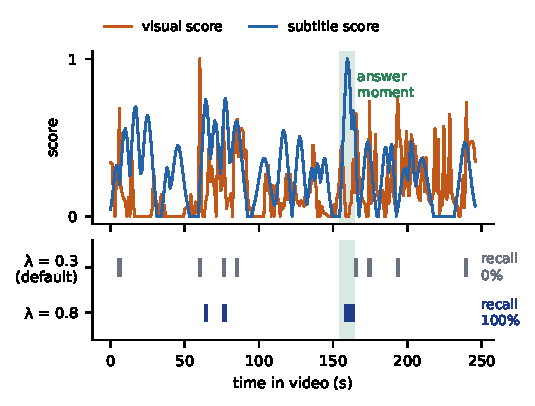
\includegraphics[width=\linewidth]{f01_teaser.pdf}\\
      {\scriptsize Real example: $\lam=0.3$ \bad{misses} the answer moment (green), $\lam=0.8$ \good{hits} it.}
    \end{column}
  \end{columns}
\end{frame}}

\newcommand{\titleframe}{%
{\setbeamertemplate{footline}{}\setbeamertemplate{frametitle}{}
\begin{frame}[t]\titlepage\end{frame}}}

\newcommand{\thankframe}{%
{\setbeamertemplate{footline}{}\setbeamertemplate{frametitle}{}
\begin{frame}[t]\mbzuaiThankYou\end{frame}}}
.
\usepackage{amsmath,amssymb}
\usepackage{booktabs}
\usepackage{xcolor}
\usetheme{MBZUAI}
\graphicspath{{assets/}{../figs/}}
\setbeamertemplate{navigation symbols}{}

\newcommand{\lam}{\lambda}
\newcommand{\strong}[1]{\textcolor{mbzuai-navy}{\textbf{#1}}}
\newcommand{\good}[1]{\textcolor{green!45!black}{\textbf{#1}}}
\newcommand{\bad}[1]{\textcolor{red!65!black}{\textbf{#1}}}

% ── Team and roles: edit here, all three decks update ─────────────────────
\newcommand{\roleJH}{Problem and setup; score cache and data pipeline; Q1 analysis; overall study (Q1--Q4)}
\newcommand{\roleLJ}{Continual learning experiments and analysis (Q2--Q3)}
\newcommand{\roleMA}{Downstream question-answering evaluation (Q4)}

\title[Fusion Weight for Keyframe Search]{Should the Fusion Weight Change with the Question?}
\institute[MBZUAI]{CV805 Course Project \\ Mohamed bin Zayed University of Artificial Intelligence}
\date{\today}
\titlelogos{assets/logo_dark.pdf}
\footleft{Should the Fusion Weight Change with the Question?}
\footright{\insertframenumber{} / \inserttotalframenumber}

% Team slide; #1 = JH, LJ or MA, the presenter's row is highlighted.
\usepackage{etoolbox}
\newcommand{\teamrow}[4]{% #1 key, #2 presenter key, #3 name, #4 role
  \ifstrequal{#1}{#2}%
    {\textbf{\textcolor{mbzuai-navy}{#3}} & \textbf{\textcolor{mbzuai-navy}{#4}} & \textcolor{mbzuai-dark-sand}{\textbf{this talk}}}%
    {\textcolor{mbzuai-subtle}{#3} & \textcolor{mbzuai-subtle}{#4} & }}
\newcommand{\teamframe}[1]{%
\begin{frame}{Team and my part}
  \centering
  \renewcommand{\arraystretch}{1.6}
  \begin{tabular}{p{0.27\textwidth}p{0.52\textwidth}p{0.11\textwidth}}
    \toprule
    Member & Main contribution & \\
    \midrule
    \teamrow{JH}{#1}{Jianxiang He}{\roleJH} \\
    \teamrow{LJ}{#1}{Longtao Jiang}{\roleLJ} \\
    \teamrow{MA}{#1}{Makhmud Assentay}{\roleMA} \\
    \bottomrule
  \end{tabular}
\end{frame}}

% Context frame used by every talk: VSI, the weight, and the example.
\newcommand{\contextframe}{%
\begin{frame}{Background: two clues, one weight}
  \begin{columns}[c,onlytextwidth]
    \begin{column}{0.47\textwidth}
      \small
      A VLM can only look at \strong{about 8 frames} of a long video, so we must pick them well.\\[2mm]
      VSI scores every second with two clues:
      \begin{itemize}
        \item \strong{Visual}: do the question's objects appear?
        \item \strong{Subtitle}: does the subtitle match the question?
      \end{itemize}
      \[ S(t) = (1-\lam)\,\text{visual}(t) + \lam\,\text{subtitle}(t) \]
      and keeps the top 8 seconds. VSI uses \strong{$\lam=0.3$ for every question}.
    \end{column}
    \begin{column}{0.5\textwidth}
      \centering
      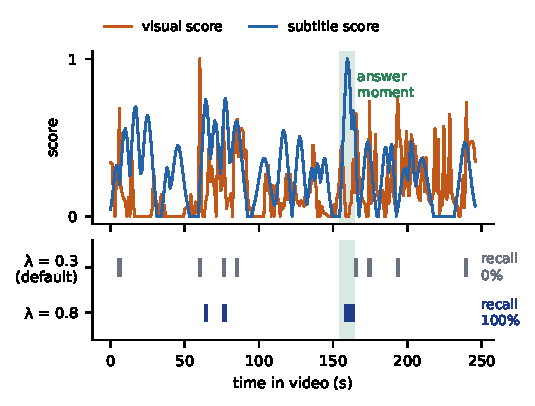
\includegraphics[width=\linewidth]{f01_teaser.pdf}\\
      {\scriptsize Real example: $\lam=0.3$ \bad{misses} the answer moment (green), $\lam=0.8$ \good{hits} it.}
    \end{column}
  \end{columns}
\end{frame}}

\newcommand{\titleframe}{%
{\setbeamertemplate{footline}{}\setbeamertemplate{frametitle}{}
\begin{frame}[t]\titlepage\end{frame}}}

\newcommand{\thankframe}{%
{\setbeamertemplate{footline}{}\setbeamertemplate{frametitle}{}
\begin{frame}[t]\mbzuaiThankYou\end{frame}}}
.
\usepackage{amsmath,amssymb}
\usepackage{booktabs}
\usepackage{xcolor}
\usetheme{MBZUAI}
\graphicspath{{assets/}{../figs/}}
\setbeamertemplate{navigation symbols}{}

\newcommand{\lam}{\lambda}
\newcommand{\strong}[1]{\textcolor{mbzuai-navy}{\textbf{#1}}}
\newcommand{\good}[1]{\textcolor{green!45!black}{\textbf{#1}}}
\newcommand{\bad}[1]{\textcolor{red!65!black}{\textbf{#1}}}

% ── Team and roles: edit here, all three decks update ─────────────────────
\newcommand{\roleJH}{Problem and setup; score cache and data pipeline; Q1 analysis; overall study (Q1--Q4)}
\newcommand{\roleLJ}{Continual learning experiments and analysis (Q2--Q3)}
\newcommand{\roleMA}{Downstream question-answering evaluation (Q4)}

\title[Fusion Weight for Keyframe Search]{Should the Fusion Weight Change with the Question?}
\institute[MBZUAI]{CV805 Course Project \\ Mohamed bin Zayed University of Artificial Intelligence}
\date{\today}
\titlelogos{assets/logo_dark.pdf}
\footleft{Should the Fusion Weight Change with the Question?}
\footright{\insertframenumber{} / \inserttotalframenumber}

% Team slide; #1 = JH, LJ or MA, the presenter's row is highlighted.
\usepackage{etoolbox}
\newcommand{\teamrow}[4]{% #1 key, #2 presenter key, #3 name, #4 role
  \ifstrequal{#1}{#2}%
    {\textbf{\textcolor{mbzuai-navy}{#3}} & \textbf{\textcolor{mbzuai-navy}{#4}} & \textcolor{mbzuai-dark-sand}{\textbf{this talk}}}%
    {\textcolor{mbzuai-subtle}{#3} & \textcolor{mbzuai-subtle}{#4} & }}
\newcommand{\teamframe}[1]{%
\begin{frame}{Team and my part}
  \centering
  \renewcommand{\arraystretch}{1.6}
  \begin{tabular}{p{0.27\textwidth}p{0.52\textwidth}p{0.11\textwidth}}
    \toprule
    Member & Main contribution & \\
    \midrule
    \teamrow{JH}{#1}{Jianxiang He}{\roleJH} \\
    \teamrow{LJ}{#1}{Longtao Jiang}{\roleLJ} \\
    \teamrow{MA}{#1}{Makhmud Assentay}{\roleMA} \\
    \bottomrule
  \end{tabular}
\end{frame}}

% Context frame used by every talk: VSI, the weight, and the example.
\newcommand{\contextframe}{%
\begin{frame}{Background: two clues, one weight}
  \begin{columns}[c,onlytextwidth]
    \begin{column}{0.47\textwidth}
      \small
      A VLM can only look at \strong{about 8 frames} of a long video, so we must pick them well.\\[2mm]
      VSI scores every second with two clues:
      \begin{itemize}
        \item \strong{Visual}: do the question's objects appear?
        \item \strong{Subtitle}: does the subtitle match the question?
      \end{itemize}
      \[ S(t) = (1-\lam)\,\text{visual}(t) + \lam\,\text{subtitle}(t) \]
      and keeps the top 8 seconds. VSI uses \strong{$\lam=0.3$ for every question}.
    \end{column}
    \begin{column}{0.5\textwidth}
      \centering
      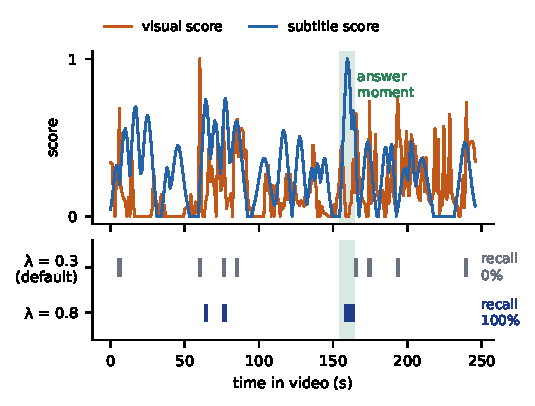
\includegraphics[width=\linewidth]{f01_teaser.pdf}\\
      {\scriptsize Real example: $\lam=0.3$ \bad{misses} the answer moment (green), $\lam=0.8$ \good{hits} it.}
    \end{column}
  \end{columns}
\end{frame}}

\newcommand{\titleframe}{%
{\setbeamertemplate{footline}{}\setbeamertemplate{frametitle}{}
\begin{frame}[t]\titlepage\end{frame}}}

\newcommand{\thankframe}{%
{\setbeamertemplate{footline}{}\setbeamertemplate{frametitle}{}
\begin{frame}[t]\mbzuaiThankYou\end{frame}}}

\subtitle{Part 3: Do Better Frames Give Better Answers? (Q4)}
\author[Makhmud Assentay]{Makhmud Assentay \\ \small with Jianxiang He and Longtao Jiang}
\footmid{Makhmud Assentay}

\begin{document}
\titleframe
\teamframe{MA}
\contextframe

\begin{frame}{My part: does it help answers?}
  \begin{columns}[T,onlytextwidth]
    \begin{column}{0.5\textwidth}
      \begin{itemize}
        \item Our team changed $\lam$ to pick frames that \strong{hit the answer moment} more often (recall@8).
        \item But the real goal is \strong{answering the question}.
        \item Recall@8 is only a stand-in: does it predict accuracy?
      \end{itemize}
    \end{column}
    \begin{column}{0.46\textwidth}
      \begin{block}{My part (Q4)}
        Built and ran the question-answering evaluation: every frame choice is given to a real VLM, and accuracy is compared on the same questions.
      \end{block}
    \end{column}
  \end{columns}
\end{frame}

\begin{frame}{How we test answers}
  \begin{columns}[T,onlytextwidth]
    \begin{column}{0.5\textwidth}
      \small
      \begin{itemize}
        \item \strong{Model}: Qwen3-VL-8B-Instruct
        \item \strong{Input}: the 8 chosen frames, each with the subtitle shown at that moment, then the multiple-choice question
        \item \strong{Output}: one option letter
        \item \strong{Frame choices}: even spacing, $\lam=0, 0.3, 0.7, 1$, oracle $\lam$, learned predictors
        \item 753 questions; learned predictors on their own test questions (3$\times$229), \strong{paired} with the default
        \item Same frames $\Rightarrow$ one model call: 3,482 calls in total
      \end{itemize}
    \end{column}
    \begin{column}{0.46\textwidth}
      \begin{exampleblock}{Prompt format}
        \scriptsize\ttfamily
        Frame 1 (12s): [image]\\
        Subtitle: \ldots\\
        \ldots\\
        Frame 8 (231s): [image]\\
        Question: \ldots\\
        A. \ldots\quad B. \ldots\quad C. \ldots\\
        Answer with the option's letter from the given choices directly.
      \end{exampleblock}
    \end{column}
  \end{columns}
\end{frame}

\begin{frame}{Result: same accuracy as default}
  \begin{columns}[c,onlytextwidth]
    \begin{column}{0.48\textwidth}
      \centering\small
      \begin{tabular}{lc}
        \toprule
        Frames chosen by & QA accuracy \\
        \midrule
        Even spacing & 0.615 \\
        $\lam=0$ (picture only) & 0.604 \\
        \rowcolor{mbzuai-light-gray}
        $\lam=0.3$ (default) & 0.631 \\
        $\lam=0.7$ (best recall) & 0.627 \\
        $\lam=1$ (subtitles only) & 0.615 \\
        Oracle $\lam$ & 0.649 \\
        \midrule
        LwF predictor (paired) & +0.4 \\
        \bottomrule
      \end{tabular}
      \par\vspace{1mm}{\scriptsize 95\% CI $[-1.5,+2.3]$, McNemar $p=0.77$}
    \end{column}
    \begin{column}{0.48\textwidth}
      \begin{itemize}
        \item Learned $\lam$ = default (\strong{+0.4}, not significant)
        \item Even the oracle adds only \strong{1.8}
        \item $\lam=0.7$ has the best recall but answers slightly \bad{worse}
        \item Using both clues beats either one alone
      \end{itemize}
    \end{column}
  \end{columns}
\end{frame}

\begin{frame}{Frames matter, for some questions}
  \centering
  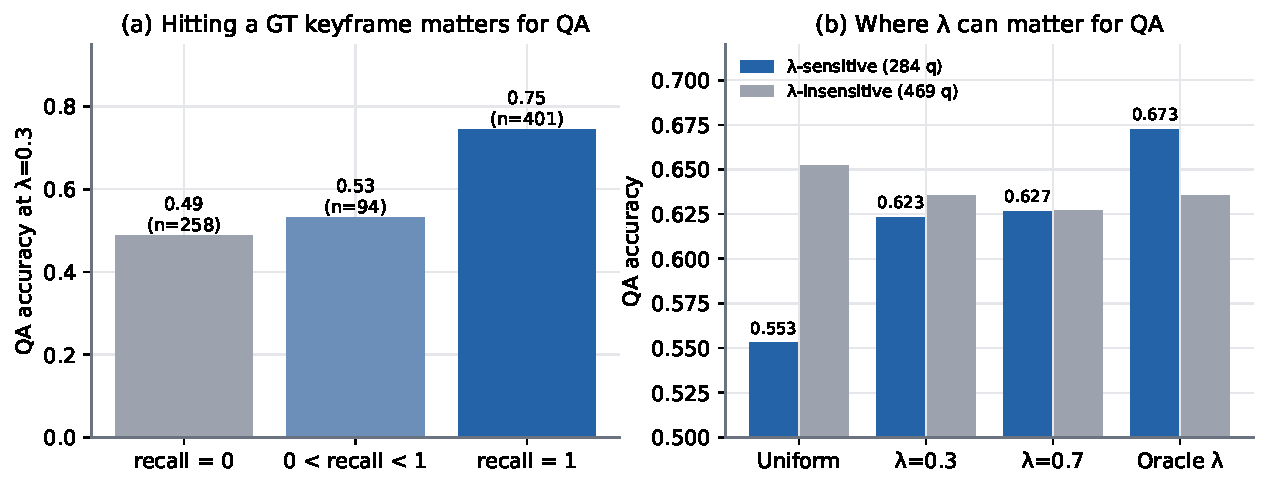
\includegraphics[width=0.84\textwidth]{f15_qa_recall.pdf}
  \par\vspace{1mm}
  \small (a) Accuracy \strong{0.49} when the 8 frames hit no answer moment vs.\ \strong{0.75} when they hit all.\\
  (b) On the \strong{284} questions where $\lam$ changes the frames, the oracle $\lam$ answers \good{5 points} more; elsewhere nothing changes.
\end{frame}

\begin{frame}{Why recall is not accuracy}
  \begin{columns}[T,onlytextwidth]
    \begin{column}{0.48\textwidth}
      \begin{block}{Reasons}
        \begin{enumerate}
          \item Only \strong{38\%} of questions react to $\lam$ at all.
          \item Recall@8 is coarse: about 2 answer moments per question.
          \item The VLM often answers from subtitles or common sense (even spacing: 0.615).
        \end{enumerate}
      \end{block}
    \end{column}
    \begin{column}{0.48\textwidth}
      \begin{alertblock}{On the 284 sensitive questions}
        LwF predictor: \strong{+1.5} over the default, but 95\% CI $[-2.3,+5.6]$ includes 0. It captures only a small part of the 5-point room.
      \end{alertblock}
    \end{column}
  \end{columns}
\end{frame}

\begin{frame}{Takeaways from Q4}
  \begin{enumerate}
    \item On all questions, a learned weight gives \strong{the same answers} as the default.
    \vspace{2mm}
    \item Frames still matter: hitting the answer moment raises accuracy from 0.49 to 0.75.
    \vspace{2mm}
    \item The weight matters only for the \strong{38\%} of questions where it changes the frames; there the best weight adds 5 points.
    \vspace{2mm}
    \item Lesson: report \strong{answer accuracy}, not only recall, and look at the questions where the change actually applies.
  \end{enumerate}
\end{frame}

\thankframe

% ════════════════════════════ backup for Q&A ════════════════════════════
\appendix

\begin{frame}{Backup: accuracy per type}
  \centering
  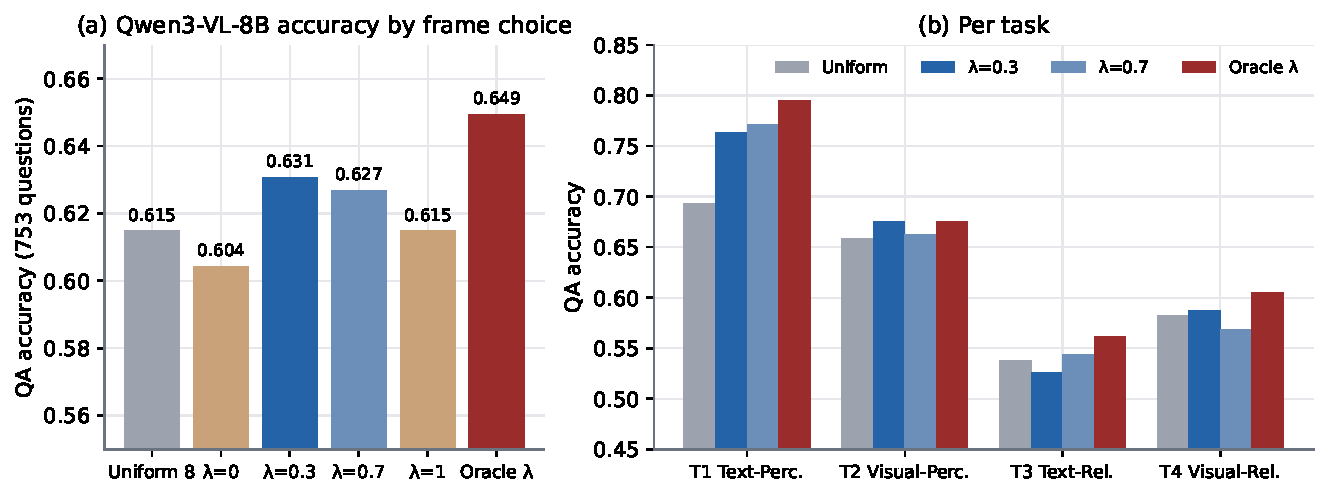
\includegraphics[width=0.9\textwidth]{f14_qa.pdf}
  \par\small\begin{tabular}{lcccc}
    \toprule
    & T1 text perc. & T2 visual perc. & T3 text rel. & T4 visual rel. \\
    \midrule
    $\lam=0.3$ & 0.764 & 0.675 & 0.526 & 0.587 \\
    Oracle $\lam$ & 0.795 & 0.675 & 0.561 & 0.606 \\
    \bottomrule
  \end{tabular}
\end{frame}

\begin{frame}{Backup: significance tests}
  \small
  \begin{itemize}
    \item Each predictor is tested on the 229 test questions of its own split, so it never saw them in training.
    \item \strong{Paired}: on exactly the same questions as the default $\lam=0.3$.
    \item LwF vs.\ default over 3$\times$229 questions: 24 questions only LwF got right, 21 only the default got right.
    \item \strong{McNemar test} on these disagreements: $p=0.77$. \strong{Bootstrap} 95\% CI of the difference: $[-1.5,+2.3]$ points.
    \item Details: bf16, at most 448$\times$448 pixels per frame, greedy decoding, subtitles within $\pm$1 s of each frame.
  \end{itemize}
\end{frame}

\begin{frame}{Backup: annotation frame rate}
  \centering
  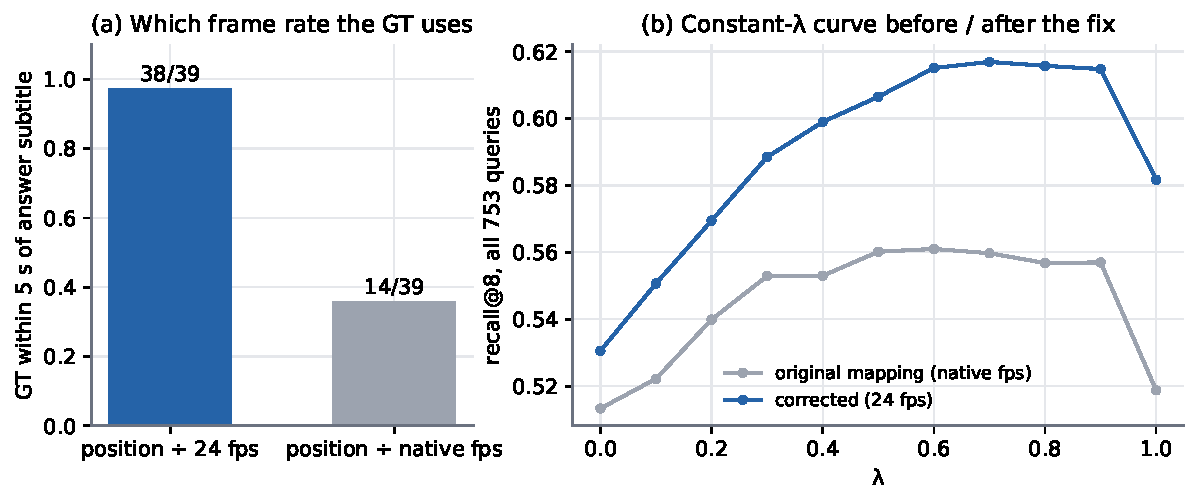
\includegraphics[width=0.85\textwidth]{f08_gtfix.pdf}
  \par\small LongVideoBench counts annotated frames at a fixed 24 fps, not the real 30 fps. (a) 38/39 annotations match the answer subtitle at 24 fps, only 14/39 at the real rate. (b) Recall vs.\ $\lam$ before and after the fix.
\end{frame}

\begin{frame}{Backup: recall vs.\ $\lam$}
  \centering
  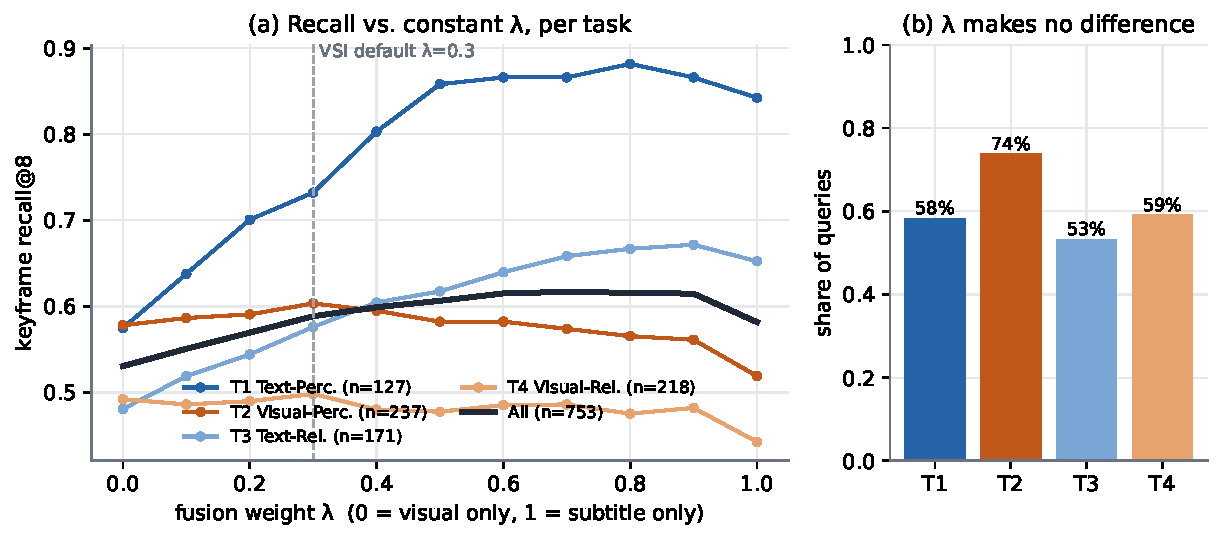
\includegraphics[width=0.85\textwidth]{f02_headroom.pdf}
\end{frame}

\end{document}
